    {
        Աշխատանքի սկզբնական փուլում կատարվել է արդեն գոյություն ունեցող կոդի ստատիկ վերլուծություն կատարող գործիքների
        ուսումնասիրություն։ Արդյունքում հետազոտվել են առաջատար գործիքների մշակված ալգորիթմների թերություններն ու
        առավելությունները, որոշ գործիքներ փորձարկվել են Ջուլիետ թեստային հավաքածույում՝ CWE-401 տիպի սխալներ\cite{CWE401} գտնելու համար։

        \subsubsection{SMOKE}
        SMOKE\cite{Fan2019}-ի ալգորիթմը կազմված է երկու հիմնական փուլերից՝ բարձր ճշտության և մասշտաբայնության հասնելու համար։
        Առաջին փուլում այն օգտագործում է պարզ, բայց ոչ ճշգրիտ վերլուծություն՝ հիշողության արտահոսքի բոլոր հնարավոր ուղիները
        հայտնաբերելու համար և զտում է այն ուղիները, որոնք չեն կարող հանգեցնել արտահոսքի: Այս նպատակով նախ օգտագործվում է նոսր
        արժեքների կախվածության գրաֆը, ապա կառուցվում է օգտագործման կախվածության գրաֆը(UFG): UFG-ն պարունակում է վերլուծության
        համար բավարար ինֆորմացիա բոլոր դինամիկ հիշողության օբյեկտների մասին։ UFG-ի յուրաքանչյուր կող համապատասխանեցվում է պայմանների հետ,
        որոնցից կախված ուղղորդվում է ծրագրի աշխատանքի ընթացքը։
        Նկար \ref{fig:figure1}-ում(վերցված է\cite{Fan2019}-ից) պատկերված է UFG-ի օրինակ։ UFG-ն բացահայտ նկարագրում է ցուցիչի արժեքների հնարավոր
        ընթացքն ստեղծելով սահմաններից դուրս գտնվող գագաթ(p@s8)։ Դա նշանակում է, որ դինամիկ հիշողության օբյեկտը, որն
        օգտագործվում էր վերը նշված ցուցիչի միջոցով այլևս հասցեավորված չէ։

        \begin{figure}[h]
            \centering
            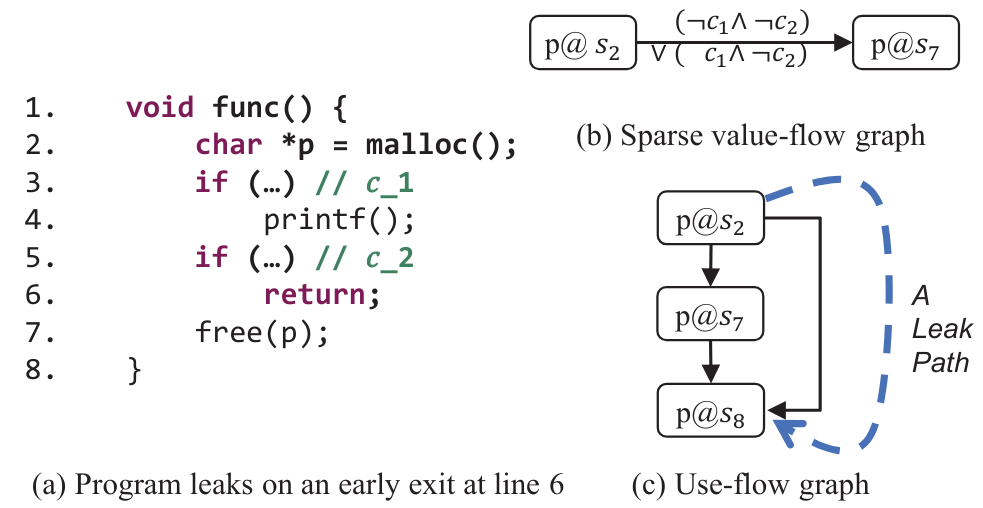
\includegraphics[width=0.6\textwidth]{pic1}
            \caption{Դինամիկ հիշողության արտահոսքի օրինակ}
            \label{fig:figure1}
        \end{figure}

        Երկրորդ փուլում այն օգտագործում է արդեն ստացված UFG֊ի առավել ճշգրիտ վերլուծություն։ Սկզբում որոնում է բոլոր
        ճանապարհները, որոնք չեն պարունակում դինամիկ հիշողություն օգտագործող օպերացիաներ։ Այնուհետև հայտնաբերված յուրաքանչյուր
        ճանապարհի համար կիրառում է Z3 գործիքը\cite{Z3}՝ նրանց իրագործելիությունը ստուգելու համար: Այս գործընթացն անհրաժեշտ է
        ճանապարհների զգայունությունն ապահովելու և կեղծ հայտնաբերված արտահոսքերը զտելու համար։ Գործիքն ունի որոշ սահմանափակումներ՝
        \begin{enumerate}[itemsep=1mm]
            \item Վերլուծությունն արվում է դաշտերի հանդեպ ոչ զգայուն։
            \item Ցուցիչների վերլուծությունը ճշգրիտ չէ։
            \item Որոշ ճանապարհներ անիրագործելի են բարդ թվաբանական և միջֆունկցիոնալ տվյալների կախվածությունների պատճառով։
            \item Հաշվի չի առնվում թվաբանական գործողությունները ցուցիչների հետ, free(p + y) արտահայտությունը համարժեք է համարվում free(p)֊ին, ինչն ակնհայտ սխալ է։
            \item Հաշվի են առվում միայն այն դեպքերը, երբ դինամիկ հիշողության առանձնացման գործողությունը բարեհաջող է անցնում։
        \end{enumerate}

        SMOKE֊ը ծրագրավորված է LLVM-ի վերին մակարդակում և միայն բինար տարբերակն է հասանելի\cite{SMOKE}:

        \subsubsection{PCA}
        CA\cite{Li2020}֊ն առաջին հերթին թարգմանում է նախնական կոդը LLVM IR֊ի։ Այնուհետև, օգտագործելով LLVM֊ի gold plugin֊ը
        բոլոր IR ֆայլերը հավաքում է մեկում։ Ապա այն օգտագործում է Անդերսենի ցուցիչների վերլուծության գործիքը\cite{Andersen}
        և հավաքում ցուցիչների մասին ինֆորմացիա, մասնավորապես, թե որ դինամիկ հիշողության օբյեկտի վրա է հղված այս կամ այն ցուցիչը։
        Այդ ինֆորմացիայի վրա հիմնվելով, կառուցվում են ֆունկցիաների կանչերի կախվածության և ղեկավարման կախվածության գրաֆները։
        Եւ վերջում, արդեն ունենալով համապատասխան գրաֆներն ու ինֆորմացիան, կառուցվում է միջֆունկցիոնալ տվյալների կախվածության գրաֆ(DDG)։

        Դինամիկ հիշողության արտահոսքի հայտնաբերման նպատակով PCA֊ը յուրաքանչյուր դինամիկ հիշողություն առանձնացնող ինստրուկցիայի(A)
        համար հավաքում է բոլոր նրանից հասանելի գագաթները(N) DDG֊ում: Եթե N֊ը առանձնացված հիշողությունն ազատող ինստրուկցիա
        չի ներառում, ապա պնդում է, որ տեղի ունի հիշողության արտահոսք։

        Որոշ դինամիկ հիշողության օբյեկտների կարող են հետևել մեկից ավելի դրանք ազատող ինստրուկցիաներ DDG֊ում։
        Նման դեպքերում, A֊ն կհամարվի ազատված, եթե գոյություն ունի ղեկավարման կախվածության ճանապարհ A֊ից դեպի այն ազատող
        ինստրուկցիան։ Հակառակ դեպքում նույնպես պնդում է, որ տեղի ունի հիշողության արտահոսք։ Գործիքն ունի հետևյալ սահմանափակումները՝
        \begin{enumerate}[itemsep=1mm]
            \item Վերլուծությունն արվում է հոսքի, դաշտի և համատեքստի հանդեպ ոչ զգայուն։
            \item Այն օգտագործում է LLVM gold plugin֊ը IR ֆալերը մեկում հավաքելու համար, այնուհետև կառուցում է DDG, ինչը գործիքը դարձնում է ոչ մասշտաբային։
            Գործիքի նախնական կոդը հասանելի է\cite{PCA}։
        \end{enumerate}

        \subsubsection{SVF}
        SVF\cite{Sui2016}֊ն հիմնված է LLVM֊ի վերին մակարդակում։ Առաջին քայլում այն թարգմանում է նախնական կոդը LLVM IR֊ի։
        Այնուհետև, օգտագործելով LLVM֊ի gold plugin֊ը բոլոր IR ֆայլերը հավաքում է մեկում։ SVF֊ն օգտագործում է որոշ ցուցիչների
        անալիզատորներ, ցուցիչների համար համապատասխան ինֆորմացիա հավաքելու նպատակով, մասնավորապես, թե որ դինամիկ հիշողության
        օբյեկտի վրա է հղված այս կամ այն ցուցիչը։ Անալիզատորներցի մեկն Անդերսենի ցուցիչների անալիզատորն է\cite{Andersen}։
        Օգտագործելով LLVM IR֊ը և ցուցիչների մասին հավաքված ինֆորմացիան՝ գործիքը կառուցում է ղեկավարման կախվածության գրաֆ(CFG)
        և հավաքում է հիշողության ստատիկ առանձին վերագրման մասին ինֆորմացիան(SSA - Static Single Assignment)։
        Յուրաքանչյուր VFG֊ի գագաթ իրենի ներկայացնում է ծրագրի որևէ ինստրուկցիա, իսկ գագաթների միջև կողերը տեղադրվում են
        օգտվելով օգտագործման֊հայտարարման և ցուցիչների մասին հավաքված ինֆորմացիայից։

        Բացի այդ, SVF-ն ապահովում է հիշողության տարածքների տարանջատում, ինչը թույլ է տալիս օգտվողներին հիշողությունը բաժանել
        հավաքածուների: Սա օգտակար է մեծածավալ ծրագրերը վերլուծելու համար, եթե հաշվի է առնվում հիշողության որոշակի տարածք:

        Տարբեր ստուգման գործիքներ կարող են իրականացվել VFG֊ի հիման վրա, որը հասանելի է օգտվող ծրագրերի համար:
        Հիշողության արտահոսքի հայտնաբերումը համարվում է աղբյուր-ստացողի խնդիր (յուրաքանչյուր հիշողության հատկացում
        յուրաքանչյուր ուղու վրա պետք է հասնի իր ազատմանը): Ստորև նշված են գործիքի որոշ սահմանափակումներ՝
        \begin{enumerate}[itemsep=1mm]
            \item Այն օգտագործում է LLVM gold plugin֊ը IR ֆալերը մեկում հավաքելու համար, այնուհետև կառուցում է DDG,
            ինչը գործիքը դարձնում է ոչ մասշտաբային։
            \item Վերլուծությունն արվում է ճանապարհների և դաշտերի հանդեպ ոչ զգայուն։
        \end{enumerate}
    }